\documentclass[french,12pt,notitlepage]{report}
\usepackage[utf8]{inputenc}
\usepackage[T1]{fontenc}
\usepackage{lmodern}
\usepackage[a4paper]{geometry}
\usepackage[francais]{babel}
\usepackage{graphicx}


\begin{document}
	\title{Functional data analysis applied to neurology}
	\author{Clément Bonvoisin, Pierre Ludmann}
	\date{30 juin 2014}
	\maketitle

	\begin{abstract}
  
Il s'agit de segmenter des signaux de marche,
dans le cadre d'une collaboration du CMLA (ENS Cachan) et Cognac-G (Paris V).
%Quels sont les travaux déjà accomplis dans ce domaine dans le monde?

On propose donc ici des algorithmes pour détecter des ruptures.
Cela permet en aval aux médecins de mieux étudier les différentes régimes de marche.
Un algorithme efficace et rapide semble encore manquer.

Si la détection d'un unique changement trouve des implémentations reconnues,
on a cherché à généraliser à de multiples ruptures.
Aussi on a changé le paramètre de décision : on exige un nombre précis de résultats plutôt qu'un seuil de détection.

Malgré de fortes hypothèses de travail,
on obtient des résultats statisfaisants sur des signaux réels et synthétiques
bien que des améliorations restes possibles.

Son utilisation doit faire place à un apprentissage sur les segments de régime obtenus.
	
	\end{abstract}

	\tableofcontents

	\chapter{Introduction au problème}
	
		La motivation initiale de ce stage provient de la médecine, et plus particulièrement de la neurologie. Le projet, piloté par le groupe Cognac-G, vise à analyser en détail des signaux physiologiques, issus d'une expérience très simple.
	\\ \\
	Le protocole expérimental se décline comme suit :
	\begin{itemize}
		\item On place sur le patient un ensemble de capteurs : un à la tête, un à la ceinture, et un sur chaque pied. Ces capteurs sont des centrales inertielles, qui permettent une mesure de l'accélération et de la vitesse angulaire du patient.
		\item On lance l'acquisition. Pendant quelques secondes, le patient est à l'arrêt. Puis, il commence à marcher sur une dizaine de mètres, effectue un demi-tour, et fait une marche retour. Il s'arrête, et on peut alors arrêter l'acquisition.
		\item On replace alors les signaux obtenus dans un repère adapté au corps humain, formé de trois axes : l'axe antéro-postérieur, l'axe transversal (aussi appelé médio-latéral), et l'axe longitudinal (aussi appelé axe vertical).
	\end{itemize}
	
	\begin{figure}[h]
		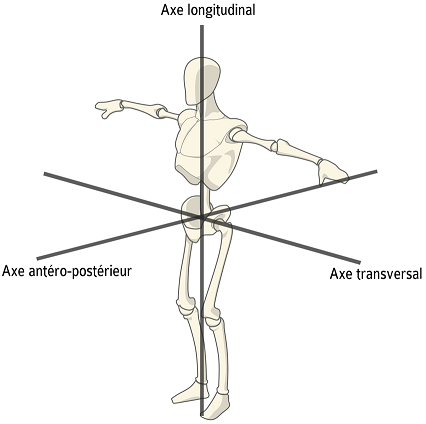
\includegraphics[scale=0.4]{axis.png}
		\caption{Le repère (antéro-postérieur; médio-latéral; vertical)}
		\label{axis}
	\end{figure}
		
	\vspace{1pc}
	
	On obtient alors des signaux physiologiques ayant 6 composantes distinctes pour chaque capteur, à une fréquence d'acquisition dépendante de la centrale inertielle utilisée ; actuellement, le projet Cognac-G dispose d'instruments permettant un échantillonnage à 100Hz.
	
	\begin{figure}[h]
		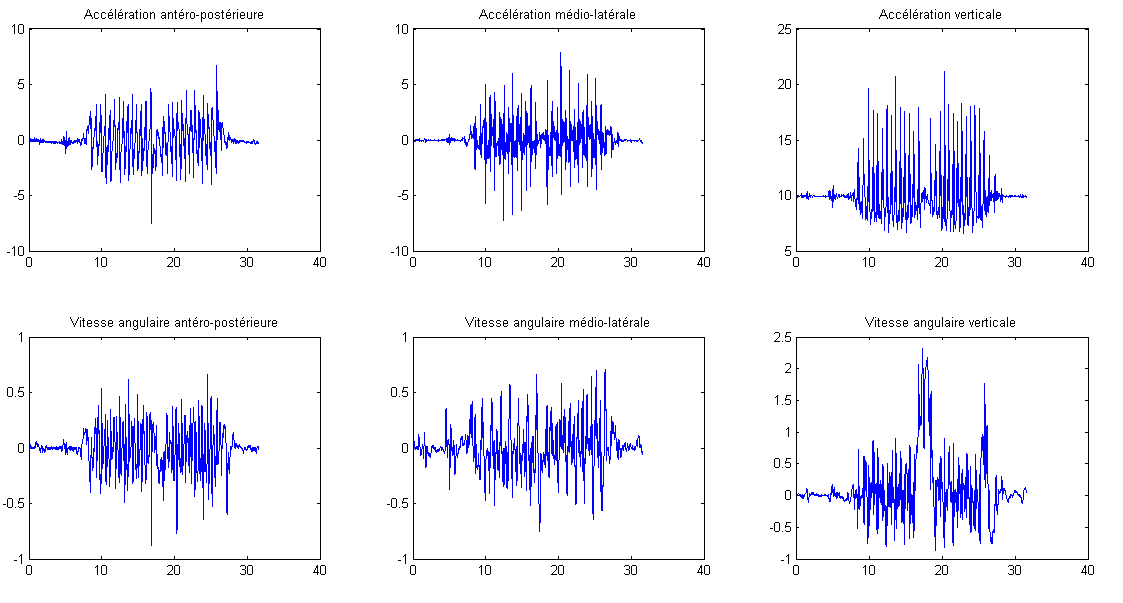
\includegraphics[scale=0.5]{ex_signal_back.png}
		\caption{Un exemple de signal de marche (enregistré à la ceinture)}
		\label{ex_signal_back}
	\end{figure}
	
	\chapter{Algorithme CUSUM : résolution du cas d'une seule rupture}
	
	\chapter{Cas de plusieurs ruptures : implémentation dichotomique}
	
	\chapter{Cas de plusieurs ruptures : implémentation par fenêtres}
	
	\chapter{Évaluation des performances}
	
	\chapter{Conclusion}
\end{document}
